\section{Proof of concept}\label{sec:proofofconcept}
The main contribution of this thesis is the theoretical foundation and development of a new approach to UI development that reduces development costs.

\subsection{Methodology}
This sections describe the methodological approach to achieve the items listed in the paragraph \ref{sec:scope}.

\subsubsection{Steps}
This section explains the methods of this analysis.

\paragraph{Definition of major design goals}
Major design goals of the UI framework are directly influenced by non-functional requirements. We consider the broader scope of UI development in order to obtain those requirements. This includes analysis of:

\begin{enumerate}
  \item the development process of UIs with web technologies
  \item contemporary frameworks and tools for UI development that enjoyed wide and rapid adoption
  \item contemporary frameworks and tools for UI development that failed
\end{enumerate}

By following what tools in \textbf{2} did right and avoiding the mistakes of tools in \textbf{3}, we define a set of design goals that the proof of concept should adhere to. We refer to the solutions and tools researched in section \ref{sec:contemporarysolutions}.

\paragraph{Specification of the proof of concept}
The section defines the architecture and design of the proof of concept. The proof of concept should demonstrate the viability of the thesis.

\paragraph{Definition of real world use cases}
By defining real world applications for the UI framework we discover user roles and user stories.

\paragraph{Implementation of proof of concept driven by use cases}
The UI framework is developed incrementally use case by use case. The major design goals are respected. We expect to gain theoretical insights while implementing both the UI framework and the HTTP APIs.

\paragraph{Evaluation of design goals}
We analyze the design goals and whether they have been met. We assess each design goal qualitatively and assign a score between 0 and 3.

\paragraph{Conclusion of approach to reduce development costs}
We break up software complexity into specific types Accidental Complexity and Essential Complexity. Both types are broken down further and the effect of using the UI framework is analyzed. We assess the change in complexity with a score between -3 and 3.

\subsection{Design goals}\label{sec:designgoals}
The following design goals should be met by the UI framework. For each design goal we discuss the goal itself, why and how we intend to meet it and how we plan to evaluate it.
The goals are partly derived by analyzing the deficits of contemporary tools to enhance UI and web development.

\subsubsection{Play nicely with others}\label{sec:playnice}
As discussed in sections \ref{graphql} and \ref{sec:soap} the fact that GraphQL and SOAP don't play nicely with others is one of their major weaknesses. Playing nicely with others is the most important design goal of the UI framework because it allows to reuse and build on top of existing research and work.
It is important to respect standards and stay compatible with existing tooling. This design goal drove the choice of JSON-LD as serialization format for \gls{linkeddata}.

We acknowledge the widespread use of HTTP and JSON as data exchange format and achieve this design goal by conforming to web standards and \textbf{extending} existing tooling. JSON-LD allows us to stay compatible with all tools consuming and producing JSON.

This design goal can be quantified by analyzing each component of the UI framework and determine whether the technologies, protocols, languages and tools for that component are either formally standardized or a defacto standard.

\subsubsection{Straightforward upgrade path}
In order to help the adoption of the UI framework it is important to show a clear upgrade path and to keep the friction of a migration at a minimum.

This can be achieved by \textbf{extending} existing standards, keeping breaking changes at a minimum and providing good documentation. Playing nicely with others helps reaching this design goal as well.

This goal can be quantified by measuring or estimating the effort to upgrade a conventional API to the suggested HATEOS API with hypermedia vocabulary.

\subsubsection{Customizability}
While providing sane defaults, the UI framework should be customizable. There should be no limitations imposed in terms of what UIs can be created.

We want to achieve this goal by allowing UI developers to override the sane defaults. They can decide to completely ignore the \gls{linkeddata} aspect and consume the HTTP API in a traditional way by hard coding knowledge into the client. The use of React as UI library allows the UI developer to pull in external React components.

This design goal is met if all possible UIs that can be drawn with conventional tools can be drawn using the UI framework.

\subsubsection{Developer ergonomics}
UI developers should be able to use the UI framework after spending minimal effort on learning.

This goal can be achieved by choosing a widely used platform that has a thriving open source community. It is important that there is an open source community for that platform because a wide adoption behind closed doors is less likely to improve developer ergonomics. \\
A big market share of the platform increases the chances that the developer is already familiar with it. The tooling of these platforms tends to be polished and battle tested. The developer is less likely to get stuck because of some edge case issues.

An established and widely adopted web stack is Node, the NPM (Node Package Manager) ecosystem together with React. This is the platform that we choose to develop the UI framework in.

\begin{table}[!htb]
  \begin{center}
    \begin{tabular}{|l|l|}
      \hline
      \textbf{ID} & \textbf{Title}\\
      \hline
      D1 & Play nicely with others \\
      \hline
      D2 & Straightforward upgrade path \\
      \hline
      D3 & Customizability \\
      \hline
      D4 & Developer ergonomics \\
      \hline
    \end{tabular}
    \caption{Overview of the 4 defined design goals.}
    \label{tab:designgoals}
  \end{center}
\end{table}

\subsection{Proof of concept for UI framework}\label{proofofconcept}
We define two real-world use cases that cover the two main capabilities of \textbf{rendering data} and \textbf{user interaction}. Each of those use cases can be implemented separately. By implementing the use cases, we develop the UI framework and respect the design goals.

The proof of concept for the UI framework consists of following components:

\paragraph{Hydra client}
The Hydra client is a wrapper around the Hydra HTTP API. It takes care of serializing Hydra resources, fetching Hydra documentation and invoking operations. The value it provides to us is mainly developer ergonomics. The most complete Hydra client is Alcaeus which we are using as a part of the UI framework.

\paragraph{Infrastructure}
The infrastructure allows UI developers to plug in their own components as renderers, it fetches data from the server using the Hydra client and it applies the renderers by providing them the data returned by the Hydra client. This component glues all other components together.

\paragraph{JSON-LD Renderer}
The JSON-LD renderer is one of the two renderers that ship with the framework. It renders the JSON-LD response as a tree and highlights keys, values and relationships.

\paragraph{Hydra Renderer}
The Hydra renderer is the second renderer that ships with the framework. It builds on top of the JSON-LD renderer and renders root resources, collections, links and operations. The Hydra renderer creates a UI on top of any Hydra API. That UI is not optimized because it has no domain knowledge.

\paragraph{Domain Renderers}
The domain renderers are provided by the UI developers. They contain domain knowledge and can only render specific data types. As discussed in section \ref{uidevelopmenttoday}, contemporary clients and their UIs are tightly coupled to HTTP APIs. \\
Domain renderers only render \gls{linkeddata} - they don't render data without context. UI developers don't hard code assumptions about the data model of the HTTP API. \\
A React component and a \gls{linkeddata} type constitute one domain specific renderer. The open-world philosophy of \gls{linkeddata} encourages reuse across company, department and team boundaries. Domain renderers can be shared together with vocabulary since they are not coupled to data models \textbf{but to \gls{linkeddata} vocabularies}.

\paragraph{Semantic UI}
Semantic UI is a set of reusable React components that constitutes the bottled up best practices of UI and UX. This is the implementation of a design language.

\begin{figure}[!htb]
  \center{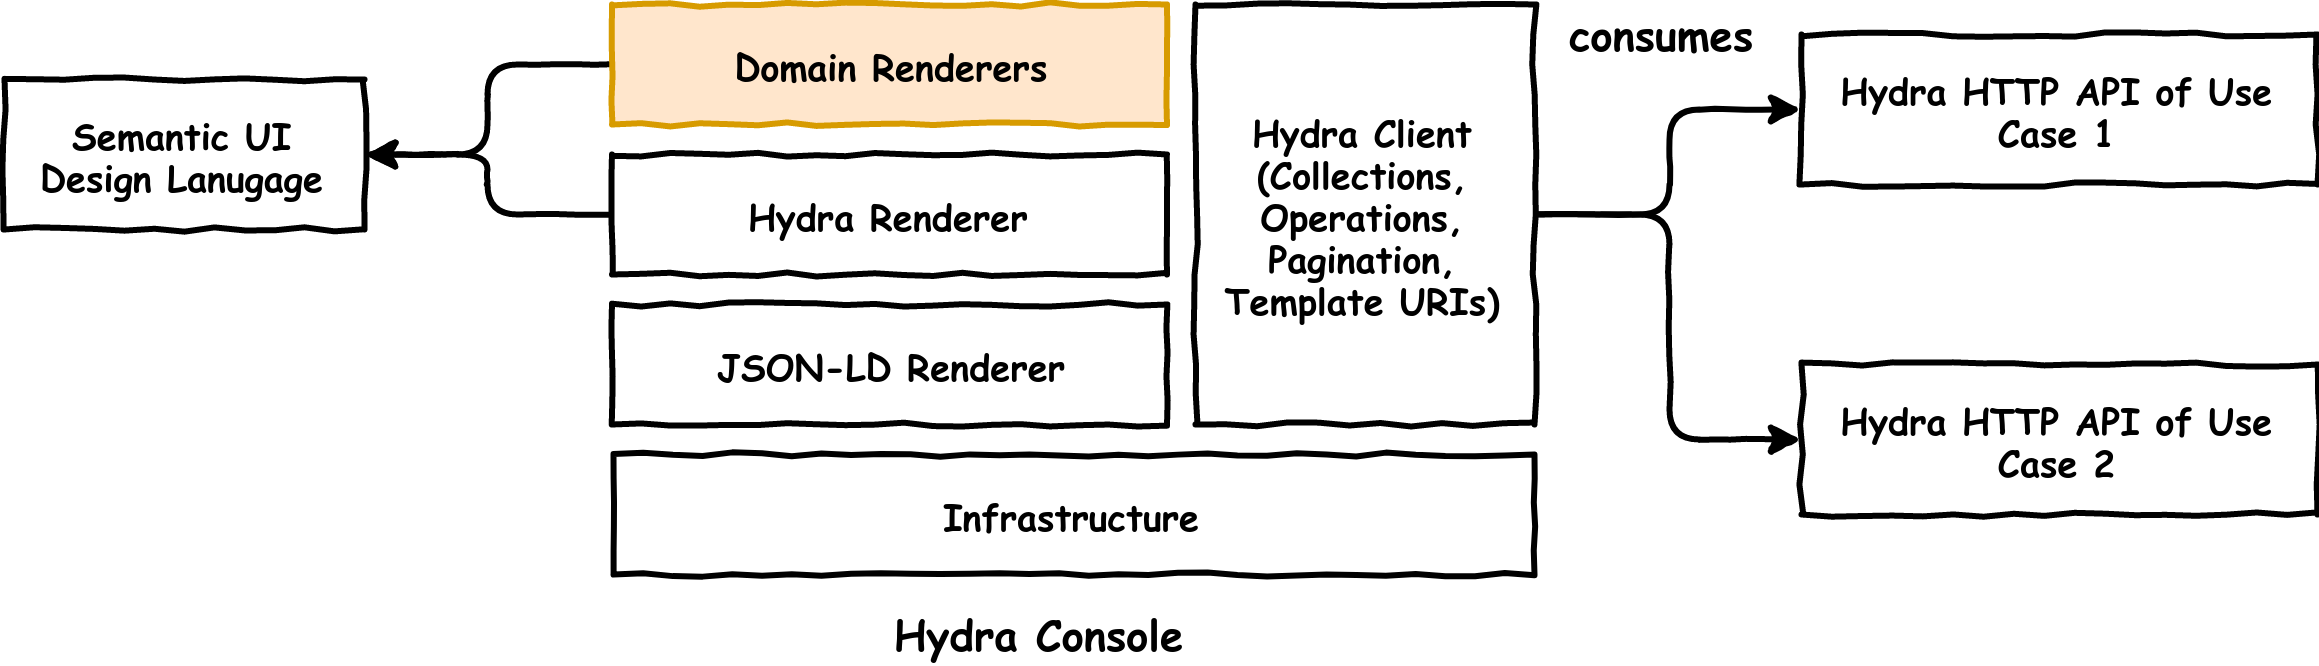
\includegraphics[width=450pt]
    {images/ui-framework-architecture.png}}
  \caption{The architecture of the proof of concept for the UI framework.}
\end{figure}

\subsection{Use Case 1: Apartment}\label{sec:usecase1}
For the user to be able to query data, the UI has to render it.

The first use case describes a scenario in home automation. Several thermometers in rooms in an apartment send the current temperature to a server. The goal is to develop a UI that displays apartments, rooms, thermometers and temperatures in a sensible manner.

\subsubsection{Requirements}

\begin{figure}[!htb]
  \center{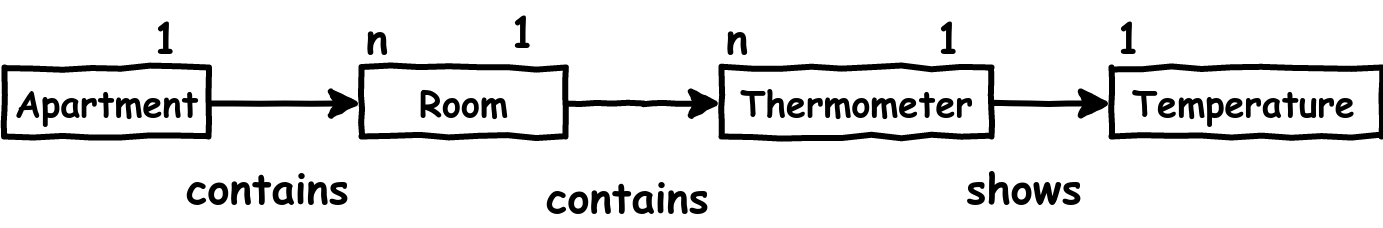
\includegraphics[width=400pt]
    {images/iot.png}}
  \caption{Data model of the apartment use case.}
\end{figure}

\begin{table}[!htb]
  \begin{center}
    \begin{tabular}{ |c|l| }
      \hline
      \textbf{ID} & \textbf{Story title} \\
      \hline
      S1 & As landlord I want to overview my apartments \\
      \hline
      S2 & As landlord I want to overview all rooms of an apartment \\
      \hline
      S3 & As landlord I want to overview thermometers of room \\
      \hline
      S4 & As landlord I want to overview the measurement data of a thermometer \\
      \hline
      S5 & As landlord I want to intuitively see the temperatures on a floor plan \\
      \hline
      S6 & As UI developer I want to present all available data without spending any development time \\
      \hline
      S7 & As UI developer I want to be able to customize the UI in order to improve it incrementally \\
      \hline
    \end{tabular}
    \caption{User stories of a scenario in home automation.}
    \label{tab:usecase1}
  \end{center}
\end{table}

\subsubsection{Hydra collection rendering}
The API exposes a collection of apartments, rooms and thermometers. Every Hydra API has an entry point and a set of root collections. These collections can be used as starting point to discover the API.

Hydra has native support for collections by using the property \lstinline{http://www.w3.org/ns/hydra/core#member}.

\lstset{language=JSON}
\begin{lstlisting}[caption=Data of /rooms as Hydra collection.]
  {
    "@context": "http://localhost:3000/iot/contexts/Room",
    "@id": "http://localhost:3000/iot/rooms",
    "@type": "Collection",
    "totalItems": 6,
    "member": [
      {
        "@id": "http://localhost:3000/iot/rooms/0",
        "@type": "https://schema.org/Room",
        "amenityFeature": "Kitchen",
        "containsPlace": [],
        "containedInPlace": "http://localhost:3000/iot/apartments/0",
        "geo": {...}
      },
      {
        "@id": "http://localhost:3000/iot/rooms/1",
        "@type": "https://schema.org/Room",
        "amenityFeature": "Laundry Storage",
        "containedInPlace": "http://localhost:3000/iot/apartments/0",
        "geo": {...}
      },
      ...
    ]
  }
\end{lstlisting}

Each member of this collection is of type \lstinline{https://schema.org/Room}. The properties can be looked up by following the URL. Given every member of the collection is of the same type, we can implement a generic renderer that looks up the properties of the member type and renders the collection as a table.

\begin{figure}[!htb]
  \center{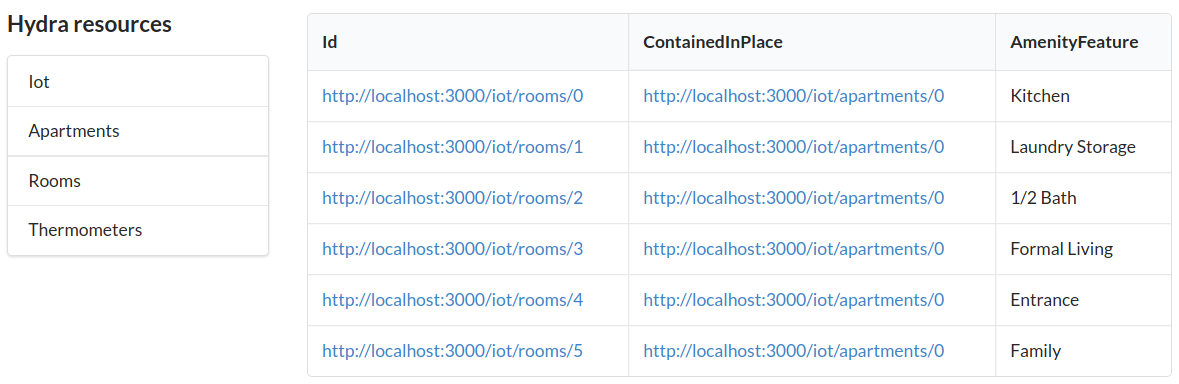
\includegraphics[width=500pt]
    {images/hydra-collections.png}}
  \caption{Generic table renderer applied on root collections.}
\end{figure}

The \lstinline{@id}s are rendered as links so that the API can be traversed by looking up resources and collections of resources.

\subsubsection{Plugin mechanism}\label{pluginmechanism}
As shown in section \ref{proofofconcept} the UI framework supports custom renderers as main mechanism to override default renderers. UI developers start out with the default set of renderers that can render arbitrary JSON-LD data and Hydra resources. \\
The fact that the API returns \gls{linkeddata} benefits this customization process. UI developers only care about rendering \textbf{certain data types}. In our use case they might be concerned with rendering the type \lstinline{Temperature}.

We demonstrate data rendering using the room \lstinline{Entrance}. The trivial JSON-LD renderer colors property keys red, properties that represent relationships blue and it renders \lstinline{@id}s as hyperlinks.

\begin{figure}[!htb]
  \center{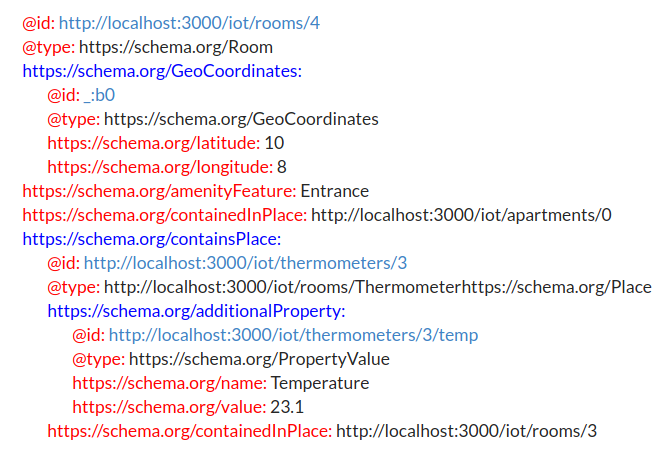
\includegraphics[width=400pt]
    {images/json-ld-renderer.png}}
  \caption{JSON-LD renderer applied on the data of \lstinline{/rooms/4}.}
\end{figure}

This room contains a list of things of type \lstinline{Thermometer} and \lstinline{https://schema.org/Place}. The thermometer has a custom \lstinline{https://schema.org/additionalProperty} that has the name \lstinline{Temperature} and a numeric value. \\
This is not straightforward to see as the JSON-LD is noisy. By applying a custom renderer to \lstinline{https://schema.org/additionalProperty} we render the temperature in one line with an icon indicating whether the temperature is hot or cold. The icon change is hard coded into the renderer.

We consider the workflow of UI developers. The UI framework expects a React component that takes the data of the \lstinline{https://schema.org/additionalProperty} and returns markup. The renderer that can be registered in the UI framework comprises of a unique id, a name, a React component and a type. The type is used by the rendering infrastructure to determine which renderers to apply on what part of the server response.

\lstset{language=JSON}
\begin{lstlisting}[caption=Renderer configuration that the developer provides.]
  {
    id: "thermometer",
    name: "Thermometer",
    comp: (data) => <Thermometer/>,
    type: "http://localhost:3000/iot/apartments/Thermometer"
  }
\end{lstlisting}

\begin{figure}[!htb]
  \center{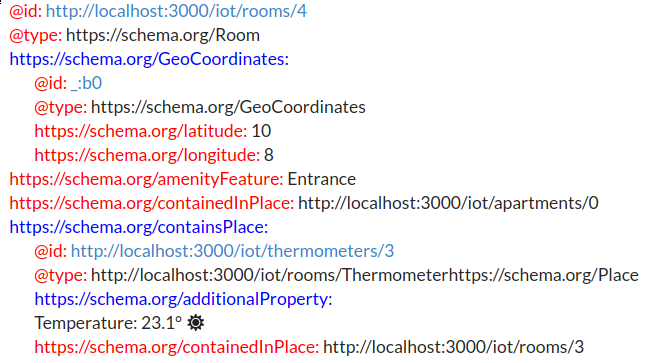
\includegraphics[width=380pt]
    {images/temperature-renderer.png}}
  \caption{The temperature renderer is applied on \lstinline{additionalProperty} on top of the JSON-LD renderer.}
  \label{fig:temperature}
\end{figure}

It is noteworthy that renderers compose by stacking them on each other. As shown in figure \ref{fig:temperature} the temperature renderer works on top the JSON-LD renderer.

By implementing similar renderers for rooms and thermometers we achieve a UI as show in figure \ref{fig:rooms}.

\begin{figure}[!htb]
  \center{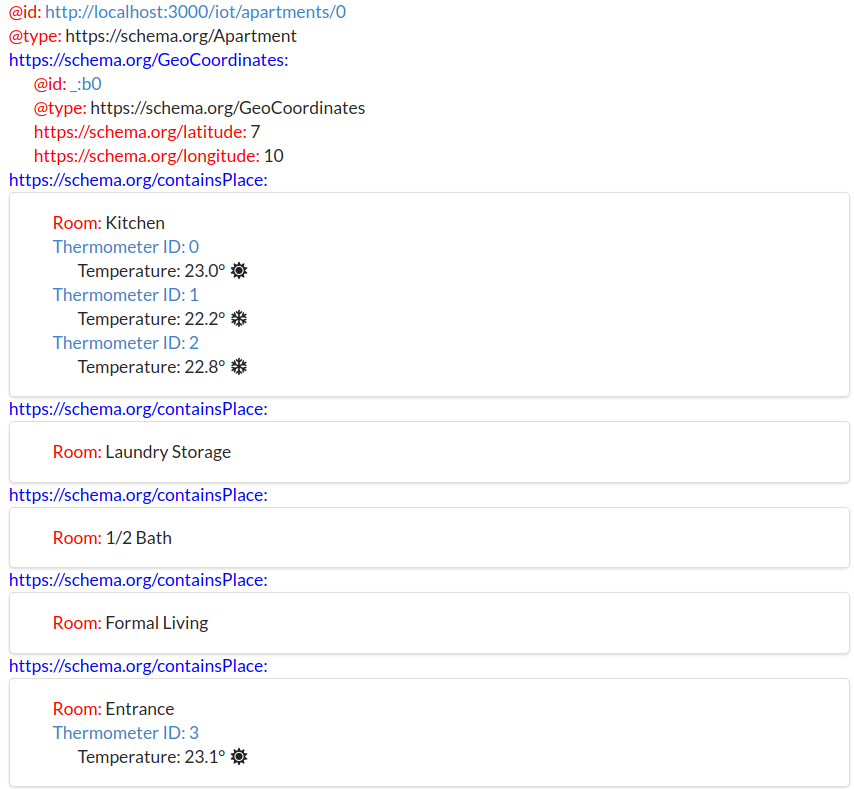
\includegraphics[width=500pt]
    {images/room-renderer.png}}
  \caption{Apartment data with active renderers: JSON-LD, Thermometer, Temperature, Room.}
  \label{fig:rooms}
\end{figure}

\subsubsection{Domain rendering}
Both default renderers are registered using the plugin mechanism. Activating both leads to a UI that is correct \footnote{Here we use the term correct in the sense of correct data rendering - the UI doesn't show wrong or non-existing data and it shows all of the response data.} and the user is able to navigate through the API using hyperlinks. This rendering setup is decoupled from the API implementation but the API has to conform to the the Hydra specification.

In order to leverage domain information for visualizing data, UI developers have to provide custom components that contain domain knowledge. We demonstrate domain rendering by looking at one apartment.

The thermometer renderer removes some noise by compacting the thermometer data. The room renderer removes some properties that are not important in this context and it draws a box around the room so they are easier to distinguish. This list view provides all information to the landlord that he cares about. \\
Places and containment relationships of places can be visualized in a more intuitive way.

\paragraph{Floor plan}
The apartment has a property called \lstinline{https://schema.org/hasMap}.

\lstset{language=JSON}
\begin{lstlisting}[caption=The \lstinline{hasMap} property of apartment /apartments/0.]
...
  "hasMap": {
  "@type": "https://schema.org/URL",
  "@id": "http://localhost:3000/iot/floorplan.jpg"
}
...
\end{lstlisting}

This property has a link to an image representing the floor plan of the apartment.

\paragraph{Geo coordinates}
All things of type \lstinline{https://schema.org/Apartment} and \lstinline{https://schema.org/Room} can have a \lstinline{geo} property.

\lstset{language=JSON}
\begin{lstlisting}[caption=The \lstinline{https://schema.org/geo} property of apartment /apartments/0.]
...
  "geo": {
    "@type": "https://schema.org/GeoCoordinates",
    "longitude": 10,
    "latitude": 7
  }
...
\end{lstlisting}

This property contains the longitude and latitude coordinates of the center of the place.

Both properties \lstinline{https://schema.org/hasMap} and \lstinline{https://schema.org/geo} are defined on the type \lstinline{https://schema.org/Place}. \lstinline{https://schema.org/Apartment} is a subtype of \lstinline{https://schema.org/Place} in the schema.org hierarchy, so our apartment renderer assumes the existence of those properties.

By leveraging coordinates of places and the floor plan of the apartment we use domain knowledge to implement a renderer that provides additional value to the landlord. By rendering the rooms on the floor plan the landlord can grasp the locations of thermometers in a more natural way.

\begin{figure}[!htb]
  \center{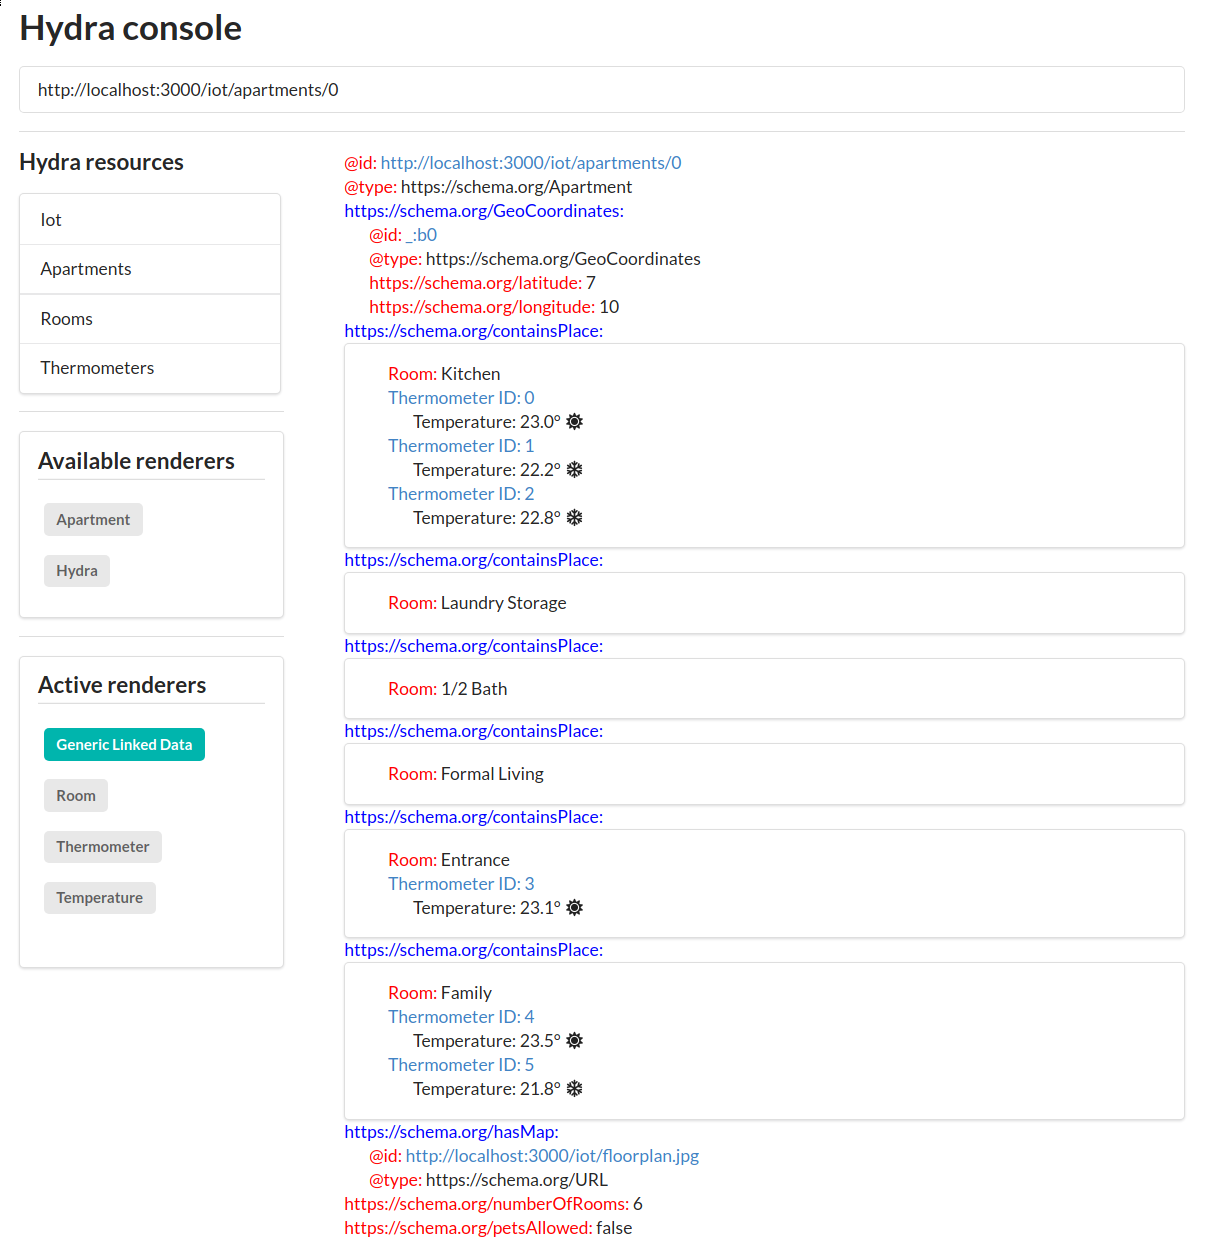
\includegraphics[width=500pt]
    {images/apartment-renderer.png}}
  \caption{Apartment data with active renderers: JSON-LD, Thermometer, Temperature, Room, Apartment, BoldFont.}
  \label{fig:apartmentrenderer}
\end{figure}

It is noteworthy that a set of renderers can be active at the same time. Whenever the rendering infrastructure encounters a data type that has a registered renderer it will apply it. In this example Hydra collections are still rendered as tables if the landlord opens the collection of rooms or thermometers.

\subsubsection{Verification of user stories}
In this section we verify that the user stories listed in table \ref{tab:usecase1} are fulfilled by either accepting or rejecting them.

\begin{table}[!htb]
  \begin{center}
    \begin{tabular}{ |l|l| }
      \hline
      \textbf{ID} & \textbf{Outcome} \\
      \hline
      S1 & Accepted: The landlord can overview the apartments \\
      \hline
      S2 & Accepted: The landlord can list all rooms of an apartment \\
      \hline
      S3 & Accepted: The landlord can list all thermometers of a rooms \\
      \hline
      S4 & Accepted: The landlord can see the temperature reported by a thermometer \\
      \hline
      S5 & Accepted: The landlord can overview the location of the temperatures on the floor plan \\
      \hline
      S6 & Accepted: The UI developer uses the default renderers to render a correct UI \\
      \hline
      S7 & Accepted: The UI developer can register custom renderers to improve the UI incrementally \\
      \hline
    \end{tabular}
    \caption{All user stories are accepted and the first use case is implemented.}
  \end{center}
\end{table}

\subsection{Use Case 2: Kanban Board}
The second use case describes a typical scenario in project management. We use this use case to explore the viability of Hydra for UIs with user interaction. A project has multiple issues which represent chunks of work. Issues can be in one of the following statuses:

\subsubsection{Requirements}

\begin{enumerate}
  \item Backlog: Status of an issue that needs additional input before it can be worked on.
  \item Ready: Status of an issue that has well defined requirements - enough information is available to start implementation.
  \item In process: Status of an issue that is being worked on.
  \item Done: Status of an issue that has been implemented.
\end{enumerate}

\begin{figure}[!htb]
  \center{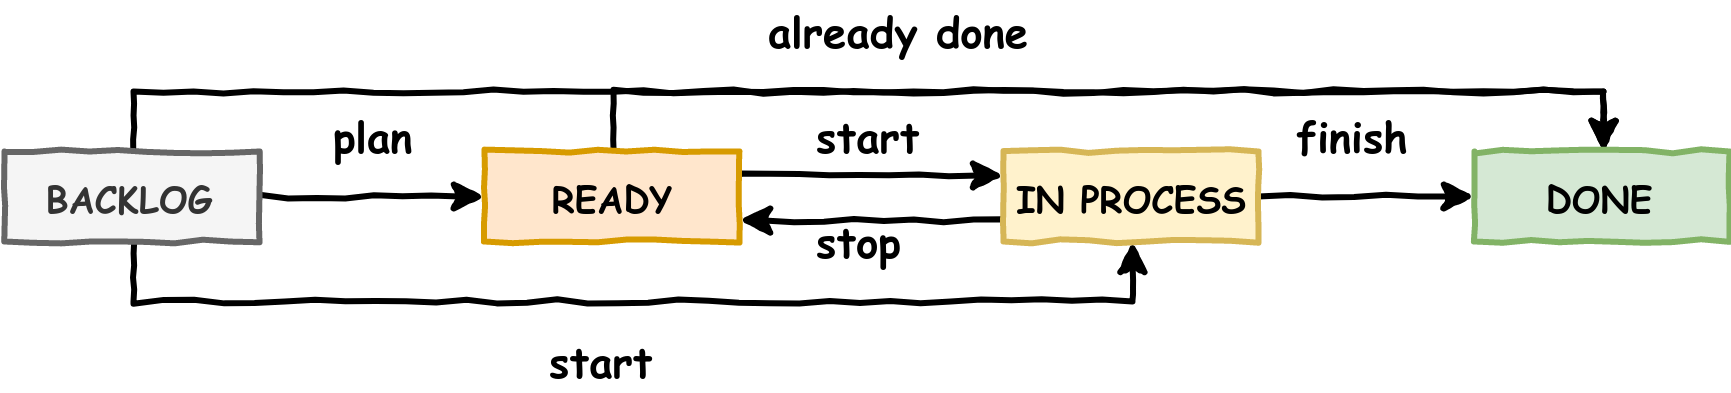
\includegraphics[width=400pt]
    {images/state-diagram.png}}
  \caption{Status transitions of an issue.}
  \label{fig:statetransition}
\end{figure}

Figure \ref{fig:statetransition} shows all possible statuses and status transitions of an issue. It is noteworthy that once an issue is ready, it can not be put back to the backlog and similarly a finished issue can not be undone.

\begin{figure}[!htb]
  \center{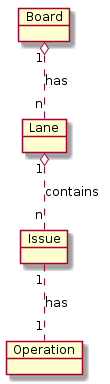
\includegraphics[width=150pt]
    {images/kanban.png}}
  \caption{Simple data model of a scenario in project management.}
\end{figure}

\begin{table}[!htb]
  \begin{center}
    \begin{tabular}{ |l|l| }
      \hline
      \textbf{ID} & \textbf{Story title} \\
      \hline
      S1 & As project manager I want to overview all projects \\
      \hline
      S2 & As project manager I want to overview all issues of a project \\
      \hline
      S3 & As project manager I want to see the status of an issue \\
      \hline
      S4 & As project manager I want to change the status of an issue \\
      \hline
      S5 & As project manager I want to remove issues \\
      \hline
      S6 & As a project manager I want to change the issue status by drag and drop \\
      \hline
      S7 & As UI developer I want to present all available data without spending time \\
      \hline
      S8 & As UI developer I want to be able to customize the UI in order to improve it incrementally \\
      \hline
      S9 & As UI developer I want to have an interactive UI without spending time \\
      \hline
    \end{tabular}
    \caption{User stories of a scenario in project management.}
    \label{tab:usecase2}
  \end{center}
\end{table}

\subsubsection{User interaction}
Hydra supports user interaction through operations. The server tells the client how to build an operation which the client then can invoke. Hydra supports three types of operations:

\paragraph{Inline operations}
The actual data is augmented with a list of supported operations. The resource has a property \lstinline{supportedOperations} where the resource is the operation object \footnote{The subject invokes the operation on an object}.

\paragraph{Attached to supported properties}
Hydra supports documentation of properties. The documentation can include information about which values are valid for a property. It is possible to attach operations to those properties.

\paragraph{Attached to supported classes}
Similar to the concept of supported properties, it is possible to document classes. Classes are used to group things together that are used the same way in certain contexts. Classes can be assigned to things by using the \lstinline{@type} property.

We attach supported operations to supported classes of issues that represent issue statuses.

\subsubsection{State transition as Hydra operations}
This section discusses the HTTP API implementation of the issue status change actions. The goal is to implement the state transition shown in figure \ref{fig:statetransition}.

\paragraph{Hydra classes}\label{par:classes}
Each status that has outgoing state transitions maps to a Hydra class. We have the classes \lstinline{BacklogIssue}, \lstinline{ReadyIssue}, \lstinline{InProcessIssue}. Note that there is no class for an issue that is done because according to the status transitions there is no way to change the status of such an issue.

Each \textbf{out} going status transition is represented by a Hydra class as well. Our API documentation contains \lstinline{IssueToReadyUpdate}, \lstinline{IssueToInProcessUpdate}, \lstinline{IssueToDoneUpdate} as additional classes. There is no \lstinline{IssueToBacklogUpdate}, because according to the state transitions, it is not possible to undo planned issues.

\paragraph{Supported operations}
Each issue class supports a list of operations.

\begin{table}[!htb]
  \begin{center}
    \begin{tabular}{ |c|l| }
      \hline
      \textbf{Status class} & \textbf{Operation classes} \\
      \hline
      BacklogIssue & IssueToReadyUpdate, IssueToInProcessUpdate, IssueToDoneUpdate \\
      \hline
      ReadyIssue & IssueToInProcessUpdate, IssueToDoneUpdate \\
      \hline
      InProcessIssue & IssueToReadyUpdate, IssueToDoneUpdate \\
      \hline
    \end{tabular}
    \caption{Status transition matrix.}
    \label{tab:statetransitionmatrix}
  \end{center}
\end{table}

Translation of the state transition diagram \ref{fig:statetransition} and mapping of the Hydra classes defined in \ref{par:classes} to the states and state transitions leads to the state transition matrix shown in \ref{tab:statetransitionmatrix}.

\lstset{language=JSON}
\begin{lstlisting}[caption=Exempt of the Hydra documentation showing the list of supported operations for the issue status class ReadyIssue.]
  ...
  {
    "@id": "http://localhost:3000/kanban/issues/ReadyIssue",
    "@type": "Class",
    "title": "Issue that is ready",
    "description": "An issue which is ready and can be started.",
    "supportedOperation": [
      {
        "@type": "http://schema.org/UpdateAction",
        "method": "POST",
        "label": "Start",
        "expects": "http://localhost:3000/kanban/issues/IssueToInProcessUpdate",
        "returns": null
      },
      ...
    ]
  },...
\end{lstlisting}

\subsubsection{Generically rendering operations}
Similar to the first use case in \ref{sec:usecase1} the list of issues is rendered using the \textit{Hydra renderer}. The properties of an issue \lstinline{description} and \lstinline{title} are columns in a table. The last column is used for Hydra operations in case any of the issues (table rows) has at least one supported operation.

Operations have an HTTP \lstinline{method} property so the client knows how to invoke that operation. We use this information to render buttons for issue removal and issue status change differently.

\begin{figure}[!htb]
  \center{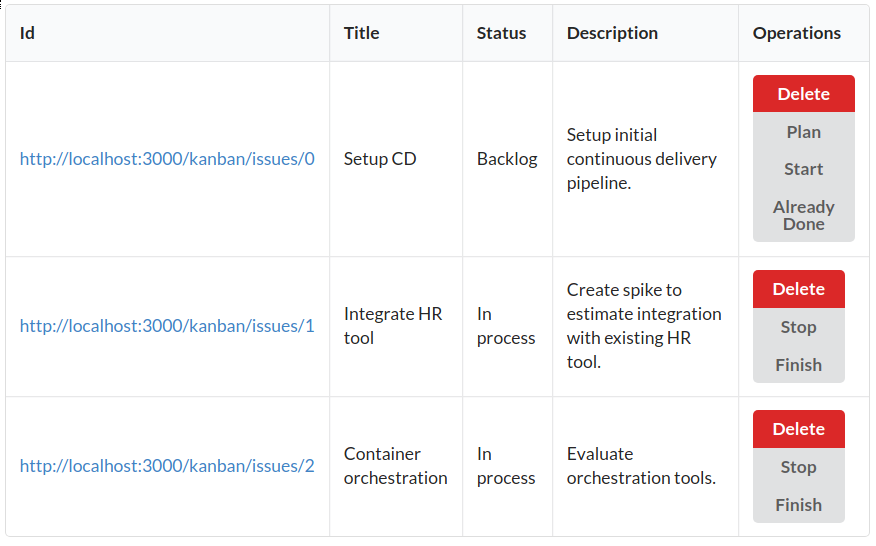
\includegraphics[width=470pt]
    {images/issues-hydra-renderer.png}}
  \caption{Collection of issues rendered by the Hydra renderer.}
  \label{fig:issueshydra}
\end{figure}

A click on a start status change button, shown in \ref{fig:issueshydra}, causes the Hydra client to invoke the operation. The client fetches \lstinline{http://localhost:3000/kanban/issues/IssueToInProcessUpdate} and sends a POST request to the URL of the issue in that row.

\subsubsection{Domain rendering}
Using the plugin mechanism mentioned in section \ref{pluginmechanism} we implement a domain specific renderer that interprets this list of issues as a Kanban \footnote{Project scheduling methodology, issue cards that move through production/development stages.} board. Figure \ref{fig:kanban} shows issues grouped by their statuses on a Kanban board.

\begin{figure}[!htb]
  \center{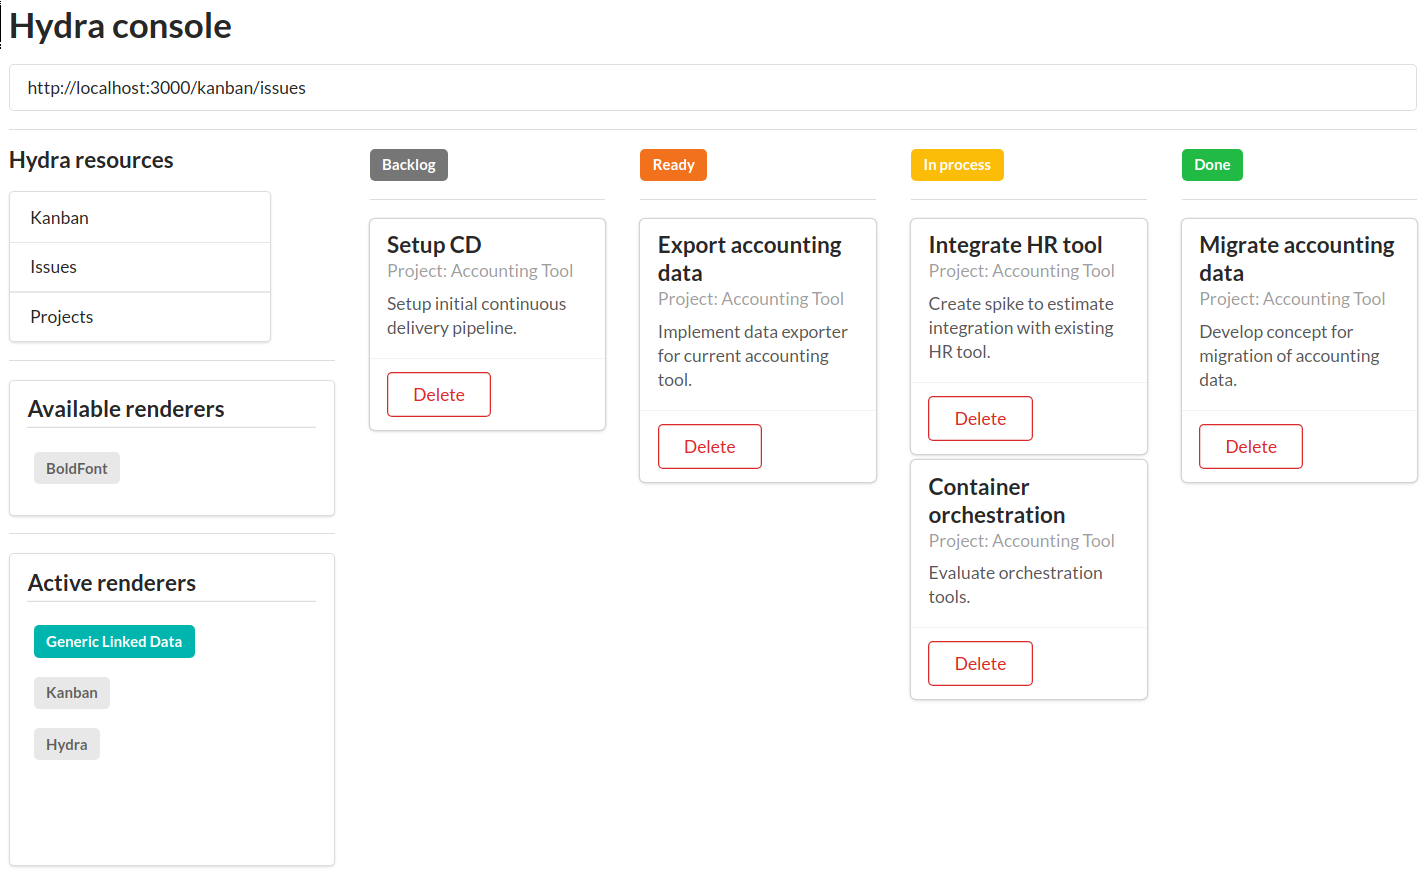
\includegraphics[width=470pt]
    {images/kanban-renderer.png}}
  \caption{Collection of issues rendered by the domain specific Kanban renderer.}
  \label{fig:kanban}
\end{figure}

\paragraph{Intuitive status change}
The Kanban renderer consumes supported operations per issue and let's the project manager invoke them in an intuitive way. The look and feel of an issue implies that it can be dropped on the target status. The visual grouping by status helps the project manager to quickly see what the development team is working on.

\paragraph{Optimistic rendering}
Optimistic rendering tries to hide the latency of the request-response life cycle. Instead of awaiting the positive response of the server confirming operation success the client behaves as if the positive response was immediate. This approach only works for operations that are expected to succeed most of the time.

For idempotent \footnote{Idempotence is a property of an operation that can be applied multiple times without changing the result beyond the initial application, in HTTP PUT and DELETE are idempotent where POST is not.} HTTP methods like \lstinline{PUT} or \lstinline{DELETE} it is possible to generically implement optimistic rendering \textbf{that works most of the time}. When the project manager for instance removes an issue, the object of the operation is known. The client immediately removes the issue from the UI without waiting for confirmation. When implementing optimistic rendering, one has to make sure to handle operation failures in a sensible way. \\
We consider the erroneous case where the project manager removes an issue and it reappears after a few hundred milliseconds. In the worst case, he doesn't pay attention after clicking the delete button and goes on thinking that the issue has been removed. This is the reason one has to carefully design optimistic rendering - especially the negative scenario. Often, it is not possible or feasible to implement optimistic rendering in a generic way.

The Kanban renderer can leverage domain knowledge to implement optimistic rendering. It simply appends the issue item to the list of issues in a column. It has knowledge of vertically aligned issue items where the Hydra renderer just knows about collections of issues. Impossible in going state transitions are communicated by not allowing issues to be dropped on the \lstinline{Backlog} column. Impossible out going state transitions are communicated by not allowing the project manager to pick up an issue that is \lstinline{Done}.

\subsubsection{Verification of user stories}
In this section we verify that the user stories listed in table \ref{tab:usecase2} are fulfilled by either accepting or rejecting them.

\begin{table}[!htb]
  \begin{center}
    \begin{tabular}{ |c|l| }
      \hline
      \textbf{ID} & \textbf{Outcome} \\
      \hline
      S1 & Accepted: The project manager can overview all projects \\
      \hline
      S2 & Accepted: The project manager can overview all issues of a project \\
      \hline
      S3 & Accepted: The project manager can see the status of an issue \\
      \hline
      S4 & Accepted: The project manager can see the status of an issue \\
      \hline
      S5 & Accepted: The project manager can remove issues \\
      \hline
      S6 & Accepted: The project manager can drag and drop issues \\
      \hline
      S7 & Accepted: The Hydra renderer shows all data \\
      \hline
      S8 & Accepted: The UI developer can override the generic renderers \\
      \hline
      S9 & Accepted: The Hydra renderer exposes all operations by default \\
      \hline
    \end{tabular}
    \caption{All user stories are accepted and the second use case is implemented.}
  \end{center}
\end{table}

\subsection{Result}
By implementing a simple dashboard for home automation and a simple Kanban board for project management, we have developed the proof of concept for the UI framework. It provides generic rendering capabilities out of the box using the JSON-LD and Hydra renderers. Those can be overridden by custom React components provided by the UI developer. Custom renderers define which \lstinline{@type}s they can render - the infrastructure takes care of rendering.

\begin{figure}[!htb]
  \center{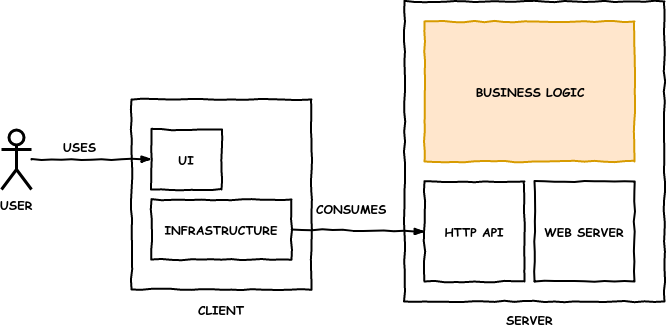
\includegraphics[width=380pt]
    {images/ui-dev.png}}
  \caption{Solely the server contains business logic.}
  \label{fig:businesslogic}
\end{figure}

Neither the client nor the custom renderers contain business rules whatsoever. The custom renderers might contain knowledge on how to present business types, but the client is merely a console to the Hydra API as shown in figure \ref{fig:businesslogic}.

\begin{figure}[!htb]
  \center{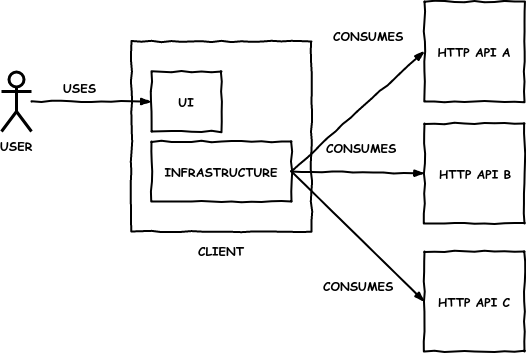
\includegraphics[width=380pt]
    {images/client-instances.png}}
  \caption{The client is decoupled from any API and is able to consume different APIs.}
  \label{fig:losecoupling}
\end{figure}

This lose coupling between client and API implementation allows the same client to be used for various API implementations as shown in figure \ref{fig:losecoupling}.

\begin{figure}[!htb]
  \center{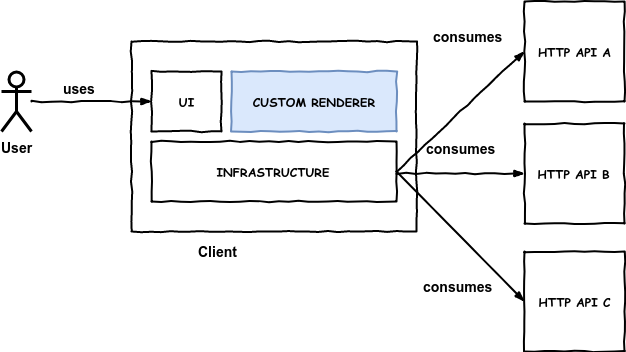
\includegraphics[width=380pt]
    {images/ui-dev-custom-renderer.png}}
  \caption{Custom renderers provide the ability to render data types. By avoiding hard coding business logic into the client the coupling to the server is still loose.}
  \label{fig:linkeddata}
\end{figure}

By using \gls{linkeddata}, custom renderers don't affect reusability of the client. A context is provided by \gls{linkeddata} so it can be understood by machines. That context is not hard coded into the client like it is often done in contemporary UI development. \\
To elaborate, we look at figure \ref{fig:linkeddata} and assume that a custom renderer for the type \lstinline{https://schema.org/Apartment} is implemented. If the responses of API A, API B and API C contain data with \lstinline{@type} \lstinline{https://schema.org/Apartment} the client can consume that data. \\
Sometimes it is required to display data differently depending on the UI context. The apartment might be rendered differently in a back office application used by administrators than an end-user facing website that lists apartments nearby. The underlying data is the same, the rendered apartment is different. This has to be resolved on the data modeling level by using Hydra classes. Classes can be used to apply additional \lstinline{@type}s depending on the context of the UI.
